\section{Keylogger}

	\subsection{Descripción}

	Se busca crear una aplicación maliciosa para Android que envíe a un atacante todo lo tipeado por el usuario, incluyendo nombres de usuario y passwords. Instalando un teclado personalizado, se puede facilmente loguear todo lo que se necesita. Sin embargo, los usuarios son cada vez más cuidadosos con lo que instalan, en parte gracias a avisos del sistema operativo informando de los peligros (ver Figura \ref{fig:keyboard}). Para que sus aplicaciones sean instaladas, los desarrolladores de teclados u otras aplicaciones de accesibilidad muchas veces no incluyen permisos de internet de tal forma de dar confianza (ver Figura \ref{fig:light_flow}).
	De esta forma, el objetivo es crear un teclado sin permisos de internet, que pueda enviar la información utilizando una segunda aplicación cómplice.
	
	\begin{figure}[h]
		\centering
		\begin{minipage}{.5\textwidth}
			\centering
			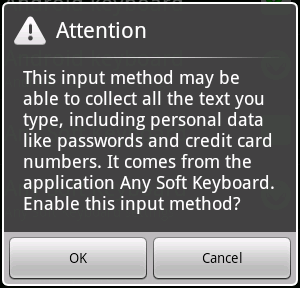
\includegraphics[width=.7\linewidth]{keyboard}
			\captionof{figure}{Warning al instalar un teclado}
			\label{fig:keyboard}
		\end{minipage}%
		\begin{minipage}{.5\textwidth}
			\centering
			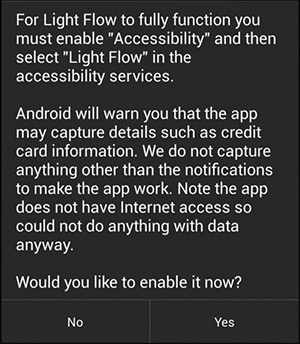
\includegraphics[width=.7\linewidth]{light_flow}
			\captionof{figure}{Ejemplo: Aplicación Light Flow avisa que sin permisos de internet no puede hacer nada con la información capturada}
			\label{fig:light_flow}
		\end{minipage}
	\end{figure}
	
	\subsection{AnimalKeyboard}
		
		\subsubsection{Permisos requeridos}
			\begin{itemize}
				\item \texttt{android.permission.BIND\_INPUT\_METHOD} Para poder registrarse como teclado. Requerido por cualquier teclado.
			\end{itemize}

		\subsubsection{Descripción}
			\emph{Animal Keyboard} es un teclado de Android que ofrece un tab de emoticones para incentivar a los usuarios a instalarlo. No tiene ning\'un permiso extra, por lo que por s\'i solo es inofensivo.	
				Al iniciarse intenta conectarse con una segunda aplicación (FunWithAnimals). Si no está instalada, no loguea nada y se comporta como cualquier teclado normal.
	
	\subsection{FunWithAnimals}
		\subsubsection{Permisos requeridos}
			\begin{itemize}
				\item \texttt{android.permission.INTERNET} Para poder bajar las fotos de animales (y enviar la información de keylogger)
			\end{itemize}
			
		\subsubsection{Descripción}
			\emph{FunWithAnimals} es una aplicación que cada vez que se abre, le ofrece al usuario una foto distinta de un gato, bajada de internet gracias a sus permisos. Si se instala por sí sola sin \emph{AnimalKeyboard}, es todo lo que hace.
			
	\subsection{AnimalKeyboard + FunWithAnimals}
	
		\subsubsection{Descripción}
		Al estar ambas aplicaciones instaladas, el procedimiento es el siguiente:
			\begin{itemize}
				\item \texttt{FunWithAnimals} registra un servicio que escucha mensajes
				\item Cada vez que se escribe una letra, \texttt{AnimalKeyboard} se la envía a \texttt{FunWithAnimals} mediante el uso de Binders \footnote{\url{http://developer.android.com/reference/android/os/Binder.html}}
				\item \texttt{FunWithAnimals} guarda las letras en un archivo
				\item Cuando el usuario abre \texttt{FunWithAnimals}, este además de bajar una foto de un gato, envía todas las letras guardadas a un servidor del atacante.
			\end{itemize}

		\subsubsection{Instrucciones}
			\begin{itemize}
				\item Instalar AnimalKeyboard.apk y FunWithAnimals.apk
				\item Ir a la configuración del teléfono
				\item Ir a Language \& input
				\item Tildar "Animal Keyboard"
				\item Ir a algún campo de texto, por ejemplo en la aplicación de SMS
				\item Arrastrar desde arriba para acceder a la barra de notificaciones
				\item Seleccionar 'Choose input method'
				\item De estar presente, apagar "Hardware physical keyboard"
				\item Activar "Animal Keyboard"
				\item El teclado nuevo debería aparecer en pantalla. Comprobar que es el correcto notando que al clickear en "123" aparece un botón nuevo de emoticones.
				\item Tipear algo
				\item Salir de la aplicación de SMS, ir al menú de aplicaciones y abrir "Fun With Animals"
				\item Se muestra en pantalla lo escrito, y se envía en segundo plano a nuestro servidor
			\end{itemize}
